Pour pouvoir transmettre les messages depuis l'utilisateur vers le téléphone portable, nous avons
choisi de mettre en place un site web à l'allure d'un gestionnaire de conversation. 
blablabla

Le fonctionnement de ce projet repose grandement sur la partie qui suit.


%%%%%%%%%%%%%%%%%%%%%%%%%%%%%%%%%%%%%%%%%%%%%%%%%%%%%%%%%%%%%%%%%%%%%%%%%%%%%%%%%%%%%%%%%%%%%%%%%%%%
\subsection{Play Framework 2.0}
%%%%%%%%%%%%%%%%%%%%%%%%%%%%%%%%%%%%%%%%%%%%%%%%%%%%%%%%%%%%%%%%%%%%%%%%%%%%%%%%%%%%%%%%%%%%%%%%%%%%

\subsubsection{primefaces vs playframework}



%%%%%%%%%%%%%%%%%%%%%%%%%%%%%%%%%%%%%%%%%%%%%%%%%%%%%%%%%%%%%%%%%%%%%%%%%%%%%%%%%%%%%%%%%%%%%%%%%%%%
\subsection{Authentification avec OAuth 2.0}
%%%%%%%%%%%%%%%%%%%%%%%%%%%%%%%%%%%%%%%%%%%%%%%%%%%%%%%%%%%%%%%%%%%%%%%%%%%%%%%%%%%%%%%%%%%%%%%%%%%%



%%%%%%%%%%%%%%%%%%%%%%%%%%%%%%%%%%%%%%%%%%%%%%%%%%%%%%%%%%%%%%%%%%%%%%%%%%%%%%%%%%%%%%%%%%%%%%%%%%%%
\subsection{Récupération des contacts google}
%%%%%%%%%%%%%%%%%%%%%%%%%%%%%%%%%%%%%%%%%%%%%%%%%%%%%%%%%%%%%%%%%%%%%%%%%%%%%%%%%%%%%%%%%%%%%%%%%%%%



\subsubsection{récupération des contacts}

\subsubsection{tri et formatage des contacts}

\subsubsection{Google cache}



%%%%%%%%%%%%%%%%%%%%%%%%%%%%%%%%%%%%%%%%%%%%%%%%%%%%%%%%%%%%%%%%%%%%%%%%%%%%%%%%%%%%%%%%%%%%%%%%%%%%
\subsection{Envoi des messages avec les websockets}
%%%%%%%%%%%%%%%%%%%%%%%%%%%%%%%%%%%%%%%%%%%%%%%%%%%%%%%%%%%%%%%%%%%%%%%%%%%%%%%%%%%%%%%%%%%%%%%%%%%%



\subsubsection{websocket}

\subsubsection{notification}



%%%%%%%%%%%%%%%%%%%%%%%%%%%%%%%%%%%%%%%%%%%%%%%%%%%%%%%%%%%%%%%%%%%%%%%%%%%%%%%%%%%%%%%%%%%%%%%%%%%%
\subsection{Design du site}
%%%%%%%%%%%%%%%%%%%%%%%%%%%%%%%%%%%%%%%%%%%%%%%%%%%%%%%%%%%%%%%%%%%%%%%%%%%%%%%%%%%%%%%%%%%%%%%%%%%%

Le design du site est l'un des thèmes que nous avons travaillé pour cette partie la du projet. 
\\
Nous souhaitions initialement avoir une interface simple, sans fioritures car cela nous semblait comme
secondaire. Nous avons donc utilisé deux frameworks pour nous faciliter la tache et accélerer la mise
en place du design.
\\
Nous avons donc tout d'abord choisi "twitter bootstrap" puis nous l'avons couplé au framework "jquery
layout".

\subsubsection{twitter bootstrap}

Twitter bootstrap est un framework web utilisé pour le développement front end. C'est un outil écrit en
Javascript et CSS qui permet de réaliser facilement des interfaces élégantes néanmoins simples. 
\\
Il nous a été utile principalement pour pouvoir concevoir l'affichage des zones d'entrée de textes ou 
encore pour organiser l'affichage des contacts proprement.
\\

\subsubsection{jquery layout}

JQuery layout est aussi un framework web. Contrairement au boostrap de twitter, il nous à permis d'organiser
notre site en plusieurs interfaces distinctes. 
\\
L'utilité de Jquery layout réside dans sa possibilité à fractionner un espace en plusieurs fenetres. Cela permet
de retrouver l'ergonomie et le coté simple et ordonné des logiciels. 
\\
Ce framework très riche nous a donc été très profitable pour pouvoir obtenir une bonne ergonomie sans avoir
à trop passer du temps sur cette partie.
\\\\

Comme le montre l'image \ref{design-final}, le couplage de ces deux frameworks a aidé à obtenir un design simple
mais effiscient. 

\begin{figure}[!h]
	\center
	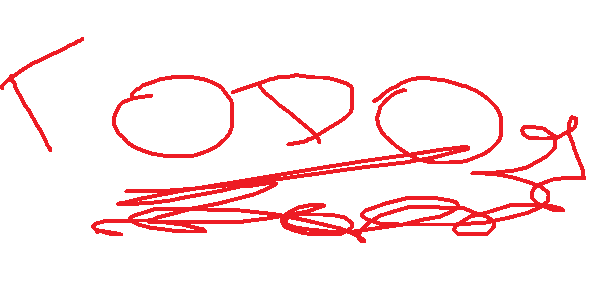
\includegraphics[width=13cm]{img/design-final.png}
	\caption{interface finale du site web}
	\label{design-final}
\end{figure}


%\begin{figure}[!h]
%	\center
%	\includegraphics[width=13cm]{img/.png}
%	\caption{}
%	\label{}
%\end{figure}
